\documentclass{beamer} 
\usepackage{amsmath,amsthm}
\usepackage{graphicx,microtype,parskip}
\usepackage{caption,subcaption,multirow}
\usepackage{attrib}

\frenchspacing

\usetheme{default}
\usecolortheme{whale}

\setbeamertemplate{navigation symbols}{}

\setbeamercolor{title}{fg=blue,bg=white}

\setbeamercolor{block title}{fg=white,bg=gray}
\setbeamercolor{block body}{fg=black,bg=lightgray}

\setbeamercolor{block title alerted}{fg=white,bg=darkgray}
\setbeamercolor{block body alerted}{fg=black,bg=lightgray}

\AtBeginSection[]
{
  \begin{frame}
    \tableofcontents[currentsection]
  \end{frame}
}

\title{}
\author{}
\institute{}
\date{}


\begin{document}

\begin{frame}
  \tableofcontents
\end{frame}


\section{How macroecology affects macroevolution: the interplay between extinction intensity and trait-dependent extinction in brachiopods.}

\begin{frame}
  \begin{block}{History}
    \begin{itemize}
      \item presented at GSA 2015
      \item rejected from \textit{Evolution}
        \begin{itemize}
          \item encouraged resubmit
          \item audience issues
          \item difficult and transformative reviews
          \item resubmitted 3 March
        \end{itemize}
    \end{itemize}
  \end{block}
\end{frame}

\begin{frame}
  \begin{block}{New measure of taxon's environmental affinity}
    Probability of observing (\# epicontinental / total \# occurrences) given Beta(\(\alpha\), \(\beta\)).
    
    \(\alpha\) is the \# epicontinental background occurrences (+ 1).
    
    \(\beta\) is the \# open ocean background (+ 1).
  \end{block}
\end{frame}

\begin{frame}
  \begin{block}{Measure of sampling and imputed values}
    Sampling is measured as the gap statistic \(r\): \\(number of bins with an occurrence - 2) / (duration in bins)

    Can only be estimated for taxa with duration of three or more. \\Have to impute (e.g. fill-in) the values for all other taxa \(r^{\ast}\).
    \begin{align*}
      r &\sim \text{Beta}(\phi, \lambda) \\
      \phi &= \text{logit}^{-1}(W\gamma) \\
      r^{\ast} &\sim \text{Beta}(\phi^{\ast}, \lambda) \\
      \phi^{\ast} &= \text{logit}^{-1}(W^{\ast}\gamma) \\
    \end{align*}
  \end{block}

  \footnotesize{Note: Beta distribution parameterized in terms of mean \(\phi\) and total count \(\lambda\). Also, this presentation excludes final (hyper)priors.}
\end{frame}
% biggest criticism was that i completely ignored effect of sampling
%   i measure sampling as the simple gap statistic
%   use it as a covariate of duration
%   this is the estimate the biasing effect of sampling
%     NOT correct duration for sampling
%     record is too coarse for a lot of methods
%     just a different way of doing it
%       i would use the new Wang approach for sampling instead of simple CLS type model
% effect of sampling probability on duration
%   (imupted) gap statistic
%   some limit pushing, but use beta regression to help estimate

% results
%   table and over-all probabilities 
%   environmental preference
%   change over time
%   covariance matrix


\section{Taxon occurrence as a function of both emergent biological traits and environmental context}

\begin{frame}
  \frametitle{Empirical questions}

  % NA doesn't have sudden faunal transitions like Eurasia

  % after \citep{Smits2015}
  %   do differences in extinction translate into differences in species pool demography?
  %     e.g. increase/decrease in occurrence over time?
  %   arboreal taxa have a greater extinction risk
  %   generalist taxa have a lower extinction risk

%   decrease in extinction risk over time
%     notice the pattern at the paleogene-neogene boundary
%   higher extinction risk in arboreal taxa
%     strong effect
%     what is variation in effect? paleogene vs neogene
%       is the transition/neogene effect so strong to appear constant?
%     driven by the environmental change?
\end{frame}

\begin{frame}
  \begin{block}{Theoretical underpinning}
    \begin{itemize}
      \item changes in demographic structure of regional species pool
      \item intersection of macroecology and macroevolution
      \item fourth-corner type problem
    \end{itemize}
  \end{block}
\end{frame}

\begin{frame}
  \frametitle{Fourth-corner problem}
% figures from papers
\end{frame}

\begin{frame}
  \frametitle{Macroevolutionary phrasing of fourth-corner problem}
% modified fourth-corner type problem
%   addition of observation, but gain of range-through
%   presence_{i,t} | individual-level_{i,t}, group-level_{t} observation_{t}
%   effects of covariates varies with t
%   instead of group-level covariates included as part of multi-level model
%   keeping in mind group-level covariates depend on t
\end{frame}


\begin{frame}
  \frametitle{Analysis of Cenozoic mammal fossil record for NA}
  \begin{columns}
    \begin{column}{0.5\textwidth}
      individual-level \\(genus i at time unit t)
      \begin{itemize}
        \item log-odds of occurrence probability at time t
        \item effect of locomotor type
          \begin{itemize}
            \item arboreal, digitigrade, plantigrade, unguligrade, fossorial, scansorial
          \end{itemize}
        \item effect of dietary type
          \begin{itemize}
            \item carnivore, herbivore, insectivore, omnivore
          \end{itemize}
        \item body size \\(rescaled log body mass)
%        \item phylogenetic effect
      \end{itemize}
    \end{column}
    \begin{column}{0.5\textwidth}
      group-level (2 My time unit t)
      \begin{itemize}
        \item overall mean of log-odds of occurrence probability
        \item temperature record based on Mg/Ca estimates
          \begin{itemize}
            \item mean and interquartile range of rescaled value
          \end{itemize}
        \item plant community phase following Graham
      \end{itemize}
    \end{column}
  \end{columns}
\end{frame}


\begin{frame}
  \frametitle{Model of taxon occurrence}
  \begin{itemize}
    \item response is p/a of genus in NA at time \(t\)
      \begin{itemize}
        \item Bernoulli variable 
        \item probability is (observation prob) times (``true'' presence)
      \end{itemize}
    \item observation probability is effect of sampling/fossil record
    \item the latent discrete ``true'' presence modeled as a \\multi-level logistic regression
      \begin{itemize}
        \item individual- and group-level
      \end{itemize}
  \end{itemize}
\end{frame}

\begin{frame}
  \begin{align*}
    y_{i,t} &\sim \text{Bernoulli}(\rho_{t} z_{i,t}) \\
    \text{logit}(\rho_{t}) &\sim \mathcal{N}(\rho^{'}, \sigma_{\rho}) \\
    z_{i,t} &\sim \text{Bernoulli}(\theta_{i, t}) \\
    \text{logit}(\theta_{i, t}) &= z_{i,t-1} (\alpha_{t} + X_{i} \beta_{t}) + (\prod_{k = 1}^{t-1} 1 - z_{i,k}) (\alpha_{t} + X_{i} \beta_{t}) \\
    \beta_{d,t} &\sim \mathcal{N}(\mu_{d}, \sigma_{d}) \\
    \alpha_{t} &\sim \mathcal{N}(\mu + \phi_{p[t]} + U_{t} \gamma, \sigma_{\mu}) \\
    \phi_{p} &\sim \mathcal{N}(0, \sigma_{\phi}) \\
  \end{align*}

  \footnotesize{Note: My implementation in Stan marginalizes over all possible (range-through) values of \(z\) instead of estimating the discrete parameters,and also uses a noncentered parameterizations of the hierarchical effects for better posterior sampling behavior. Also, this presentation excludes final (hyper)priors.}
\end{frame}

\begin{frame}
  \frametitle{Posterior predictive model checking}
  \begin{itemize}
    \item simulate fossil record given only \(y_{\_t = 1}\), all its covariates, and \(\theta\)
      \begin{itemize}
        \item where \(\theta\) is the set of all parameters
      \end{itemize}
    \item leave-one-out cross-validation for time series
      \begin{itemize}
        \item Bayesian statement is \(p(\tilde{y}_{\_(t + 1)} | y_{\_t} \theta)\)
      \end{itemize}
    \item ROC as measure of performance
  \end{itemize}
\end{frame}


\section{Other projects}

\begin{frame}
  \frametitle{How cryptic is cryptic diversity? Machine learning approaches to classifying morphological variation in the Pacific Pond Turtle (\textit{Emys marmorata})}
  \begin{itemize}
    \item estimate which species classification is best supported by morphology
      \begin{itemize}
        \item multiple machine learning approaches
        \item focus on one turtle species complex
        \item results compared against results from two other turtle datasets
        \item comparison of in- and out-of-sample model performance
      \end{itemize}
    \item collaboration with Ken, Jim Parham, and Bryan Stuart
    \item submitted to then rejected from Systematic Biology
    \item resubmitted soon
  \end{itemize}
\end{frame}

% bivalve naming rate w/ stewart
\begin{frame}
  \frametitle{Modeling the rate at which new species are named.}
  \begin{columns}
    \begin{column}{0.5\textwidth}
      \begin{itemize}
        \item collaboration with Stewart Edie; he's lead
        \item I developed the statistical model
          \begin{itemize}
            \item zero-inflated Poisson model 
            \item both Bernoulli and Poisson modeled as time series
            \item response is the number of species named per publication \\per year for each biogeographic province
          \end{itemize}
        \item targets seem to be PNAS or Systematic Biology
      \end{itemize}
    \end{column}
    \begin{column}{0.5\textwidth}
      \begin{center}
        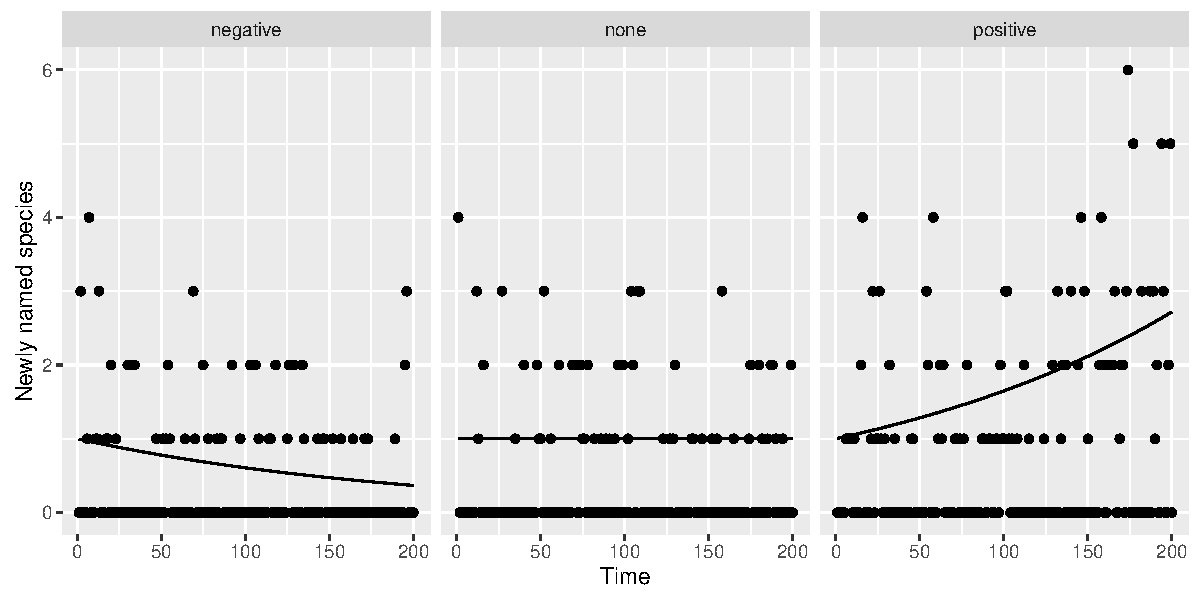
\includegraphics[width=\textwidth,height=0.8\textheight,keepaspectratio=true]{figure/prior_pred}
      \end{center}
    \end{column}
  \end{columns}
\end{frame}


\section{Moving forward}

\begin{frame}
  \frametitle{Post-doc ideas}
  \begin{enumerate}
    \item Miller Fellowship at Berkeley with Charles Marshall
      % i don't think i'm good enough for this
      \begin{itemize}
        \item Charles has met me a couple times.
      \end{itemize}
    \item Peter Buck Fellowship at Smithsonian with Gene Hunt \\(and Peter Wagner and Kate Lyons)
      % i don't think i'm good enough for this
      \begin{itemize}
        \item Gene, Pete, and Kate all know who I am.
      \end{itemize}
    \item Michigan Fellowship at University of Michigan \\with Matt Friedman
      % i don't think i'm good enough for this
      \begin{itemize}
        \item I don't know if he's actually moving there.
      \end{itemize}
    \item NIMBiOS Post-doc with Brian O'Meara
      \begin{itemize}
        \item I don't know him.
      \end{itemize}
  \end{enumerate}
\end{frame}

\begin{frame}
  \frametitle{Research program}
  % macroevolutionary macroecology
  %   macro$^{2}$
  % modeling (bayesian, hierarchical/GLMM)
  % empirical tests of macroevolutionary theories
\end{frame}



\end{document}
